\ifsvnmulti
 \svnkwsave{$RepoFile: lyapunov/Lyapunov.tex $}
 \svnidlong {$HeadURL$}
 {$LastChangedDate$}
 {$LastChangedRevision$} {$LastChangedBy$}
 \svnid{$Id$}
\fi

\chapter{Lyapunov vectors}
\label{s:LyapunovVec}

This part of the blog focuses on the use of `covariant Lyapunov
vectors' (CLV) to identify the number of degrees of freedom
that capture the physics of a `turbulent' PDE on a spatial
domain. 

As material is written up, parts of it will migrate from its
current placement into coherent sections, suitable for
inclusion into ChaosBook.org, or, God Forbid, actual {\em
publications}.

\begin{description}

\item[2009-09-04 Predrag]
Talked to  Hugues Chat\'{e}, got very
enthused about their results about splitting the KS
eigenvectors into the `physical,' inertial manifold ones,
and the `hyperbolically isolated,' transient ones. We should
reexamine eigenvectors of our solutions, might find the split
already on our very small system sizes (they work at $L=96$).

Here is my email to Chat\'{e}:

\end{description}

Iggy (as Anglos spell it),
%
now that I have become your fan - I just love all those `unphysical,'
lonely, isolated, alienated eigenvectors banished into their neurotic
transitory world off the inertial manifold -  I'm entering following
references to your papers:
\refrefs{PoGiYaMa06,ginelli-2007-99,YaTaGiChRa08,TaGiCh09}
in the final final edits of to be published in SIADS\rf{SCD07} (part I;
part II is still being penned - 60,000 relative {\po s} and no
place to go). Let me know if these are the right ones, add/correct what
needs to be edited, corrected.

I have no clue why you guys call linearized stability
eigenvectors `Lyapunov' (in My Book Lyapunov has to do with
the $J^T J$ symmetric matrix, with only real parts of Floquet
multipliers captured, and eigenvectors that do not seem to
mean anything), but you must have your reasons. We have 10-30
leading eigenvectors for our `narrow cell' with $L=22$, for
each one of the 60,000 invariant solutions that clever but
mindless computation has handed us, and nothing interesting
we had found to do with them, but they should presumably fit
into your bigger L eigenvectors as into a glove. We see
`unphysical' eigenvalues drop like a ton of rocks - only 4
leading eigenvalues really matter, 2 of them marginal at
$L=22$.

PS - for something more `physical,' check out
\HREF{http://www.warwick.ac.uk/~masax/}{Dwight Barkley}'s long pipe calculations with
\HREF{http://adsabs.harvard.edu/abs/2008APS..DFD.BD008B}{David Moxley}.
You'll find them inspirational. Probably the same story as KS, but explaining the
phase transition between frozen puffs and turbulent puffs would make plumbers happy.

\section{Reading assignments}

\noindent{\bf Predrag, to us:} Here are the relevant articles.

\begin{description}
\item[Characterizing dynamics with covariant Lyapunov
              vectors,] by
Ginelli, Poggi, Turchi, Chat\'{e}, Livi and Politi\rf{ginelli-2007-99}
is the main reference on the
`covariant Lyapunov vectors.' They describe the QR algorithm for
computing Gram-Schmidt vectors (GSV) and recovering
the covariant Lyapunov vectors (CLV) from them.
They show, using covariant Lyapunov vectors, that
  the chaotic solutions of four spatially-coupled maps,
(a) chaotic tent maps,
(b) chaotic symplectic maps,
(c) continuous time rotator model, and
(d) Fermi-Pasta-Ulam chain
  evolve within a manifold spanned by a finite number
  of physical modes.

\item[Hyperbolicity and the effective dimension] of
    spatially-extended dissipative
    systems, by Yang, Takeuchi, Ginelli, Chat\'{e}
    and Radons\rf{YaTaGiChRa08},
 is a demonstration of what we
  have observed numerically, that a finite number of Fourier modes
  captures most of the dynamics of KS, and most relevant to our research.
 They show, using covariant Lyapunov vectors, that
  the chaotic solutions of two spatially extended dissipative
  systems, \KS\ and complex Landau-Ginzburg,
  evolve within a manifold spanned by a finite number
  of physical modes hyperbolically isolated from a set of
  residual degrees of freedom, themselves individually
  isolated from each other. The number grows linearly with
  $L$ and is twice as large as the Kaplan-Yorke dimension estimates.
  The results imply that a
  faithful numerical integration of dissipative
  partial differential equations needs to incorporate at
  least all physical modes and that increasing the resolution
  beyond that
  merely increases the number of isolated modes.

\item[\bf 2009-09-16 Lyapunov vectors, illustrated.]
In order to spare you from reading the source literature, I'm including here
those figures from Yang \etal\rf{YaTaGiChRa08} that I find most striking.
The main advance of using Lyapunov vectors instead of eigenvalues alone
is that the approximate orthogonality of the `isolated' ones provides a clear
threshold between the `physical' and the rest.

You might be unimpressed by the KS example, as the $-k^4$ hyper-diffusion
term kills all higher Fourier modes very effectively. For that reason the
complex Ginzburg-Landau equation, \reffig{fig:lyapSpecCLG}
is very persuasive; the nonlinearity is
of $u(x)^3$ variety (instead of $u \partial u$ of Navier-Stokes and
KS), but there is only a $-k^2$ diffusive term, and nevertheless there
is a clear threshold for the `isolated' Lyapunov vectors. Furthermore,
the system exhibits left and right traveling waves, which is more like
fluids than the rigid wave patterns of KS.

\begin{figure}
 (a)~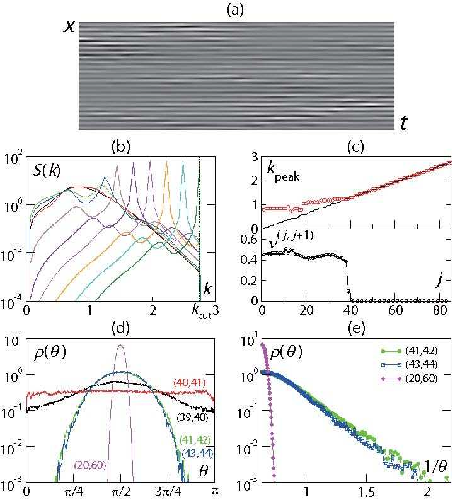
\includegraphics[width=0.45\textwidth]{../figs/YaTaGiChRa08fig2}
 (b)~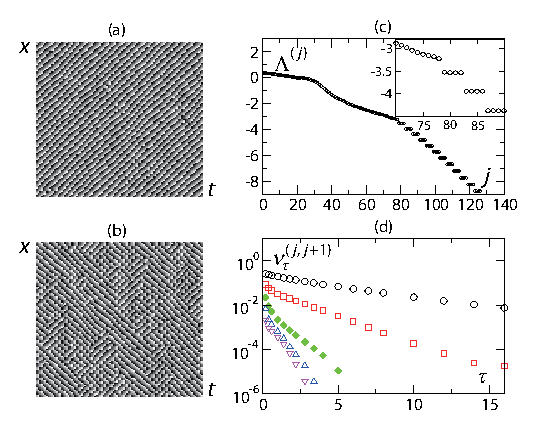
\includegraphics[width=0.45\textwidth]{../figs/YaTaGiChRa08fig3}
\caption{
(left panel)
Fig.~2 of Yang \etal\rf{YaTaGiChRa08}:
Properties of covariant Lyapunov vectors for the KS system
($L = 96$, $k_{\rm cut} = 42 \cdot 2\pi/L$, and PBC).
(a) Spatiotemporal plot of a typical vector in the isolated region
($j=46$, total time $100$).
(b) Spatial power spectra of vectors of indices
$j = 1$, $16$, $32$, $38$, $44$, $52$, $60$, $68$, $76$, $84$
(from left to right in peak position).
(c) Top panel: peak wavenumber in the power spectra (red circles)
and $k = [j/2] \cdot 2\pi/L$ (black line).
Bottom panel: DOS violation fraction $\nu^{(j,j+1)}_\tau$ for pairs of
neighboring vectors (pairs within the same step are omitted).
(d) Angle distributions between pairs of vectors.
(e) Same as (d) but with a different abscissa.
(right panel)
Fig.~3 of Yang \etal\rf{YaTaGiChRa08}:
Complex Ginzburg-Landau equation in the amplitude turbulence regime
($L = 64$, $k_{\rm cut} = 31 \cdot 2\pi/L$, and PBC).
(a,b) Spatiotemporal plots of the phase component of a typical vector $j = 91$ in the isolated region
(same trajectory, but at two distant periods of time, during a total time of $20$ for each plot).
(c) Lyapunov spectrum; inset: close-up around threshold.
(d) Time fraction $\nu^{(j,j+1)}_\tau$ of DOS violation, as a function of $\tau$
($j=78$, 82, 86, 90, 94, from top to bottom).
}
\label{fig:lyapSpecCLG}
\end{figure}



\item[Lyapunov analysis and the collective dynamics]
of large chaotic systems\rf{TaGiCh09}:
Not as directly relevant to us as \refref{YaTaGiChRa08}.
They show, using globally-coupled (a) limit-cycle oscillators
(b) noisy logistic maps, that the collective dynamics
of large chaotic systems is encoded in their Lyapunov spectra:
most modes are typically localized on a few degrees of freedom,
but some are delocalized, acting collectively on the trajectory.
For globally-coupled maps, they show moreover a quantitative
correspondence between the collective modes and some of the
so-called Perron-Frobenius dynamics.


\item[An efficient method for recovering Lyapunov vectors] from
singular vectors\rf{WoSa07}: {\bf Predrag 2009-10-15} Wolfe
and Samelson seem to be the most important article to
understand. If Ginelli \etal\rf{ginelli-2007-99} say the key
thing (how to compute covariant eigenvectors, actually) they
hide it well.
Wolfe and Samelson say: `` Standard techniques for computing
Lyapunov vectors produce results which are norm-dependent and
lack invariance under the linearized flow. An efficient,
norm-independent method for constructing the $n$ most rapidly
growing Lyapunov vectors from $n\!-\!1$ leading forward and  $n$
leading backward asymptotic singular vectors is proposed. The
Lyapunov vectors so constructed are invariant under the
linearized flow in the sense that, once computed at one time,
they are defined, in principle, for all time through the
tangent linear propagator.
	\PC{remember `the tangent linear propagator'}		\toCB
An analogous method allows the
construction of the $n$ most rapidly decaying Lyapunov vectors
from $n$ decaying forward and $n\!-\!1$ decaying backward singular
vectors. ''

\HREF{http://www.mpipks-dresden.mpg.de/~ecodyc10/Contributions/Samelson.pdf}
{This talk} might be a quick introduction to the main points of their
paper.

\item[From synchronization to Lyapunov exponents and
              back]\rf{PoGiYaMa06}:
The early paper in this series.
In the first part they discuss a general approach to determine
Lyapunov exponents from ensemble- rather than time-averages.
The approach passes through the identification of locally
stable and unstable manifolds (the Lyapunov vectors), thereby
revealing an analogy with generalized synchronization. The
method is then applied to a periodically forced chaotic
oscillator. The
analytical calculations are carried out for a model, the
generalized special flow, that they construct as a simplified
version of the periodically forced R\"ossler oscillator.

\item[Structure of characteristic {L}yapunov vectors]
in spatiotemporal chaos\rf{PaSzLoRo09}:
They study Lyapunov vectors (LVs) corresponding to
the largest Lyapunov exponents in systems with spatiotemporal
chaos. They focus on characteristic LVs and compare the results
with backward LVs obtained via successive Gram-Schmidt
orthonormalizations. Systems of a very different nature such
as coupled-map lattices and the (continuous-time) Lorenz `96
model exhibit the same features in quantitative and
qualitative terms. They propose a minimal
stochastic model that reproduces the results for chaotic
systems.

\item[The predictability of a flow] which possesses
                many scales of motion\rf{lorenz69},
AKA Lorenz 1969 36-variable method is beloved by weathermen:
we might consider using it as a test of our higher-dimensional
visualizations.

\item[Periodic orbits, Lyapunov vectors, and singular
    vectors] in the Lorenz system\rf{TrePan98}:
{\bf Predrag 2009-10-15} Trevisan and Pancotti apparently
need to be cited for the observation that covariant vectors
reduce to Floquet eigenvectors in the particular case of a
{\po} (seems so obvious it is in ChaosBook without
attribution, and Ruelle and Eckmann\rf{eckerg} surely say
that... Wolfe and Samelson\rf{WoSa07} are inspired by this
article, but seem to go beyond it. Trevisan and Pancotti say
``
A {\po} analysis in the Lorenz system
and the study of the properties of the associated tangent
linear equations are performed.
	\PC{remember `the associated tangent linear equations'}		\toCB
A set of vectors are found
that satisfy the Oseledec (1968) theorem and reduce to
Floquet eigenvectors in the particular case of a periodic
orbit. These vectors, called Lyapunov vectors, can be
considered the generalization to aperiodic orbits of the
normal modes of the instability problem and are not
necessarily mutually orthogonal. The relation between
singular vectors and Lyapunov vectors is clarified. The
mechanism responsible for super-Lyapunov growth is shown to
be related to the nonorthogonality of Lyapunov vectors. The
leading Lyapunov vectors, as defined here, as well as the
asymptotic final singular vectors, are tangent to the
attractor, while the leading initial singular vectors, in
general, point away from it. Perturbations that are on the
attractor can be found in the subspace of the leading
Lyapunov vectors.
    ''

\item[On the concept of stationary {L}yapunov basis] by Ershov
and Potapov\rf{ErshPot98}, available on
\HREF{http://www.math.ualberta.ca/~apotapov/Publications.htm}
{http://www.math.ualberta.ca/$\sim$apotapov}. They establish
existence of `stationary {L}yapunov basis'					\toCB
$\{\jEigvec[1],\cdots,\jEigvec[d]\}$ (called elsewhere `covariant
Lyapunov vectors') such that the Lyapunov
exponents are given by										\toCB
\beq
    \eigExp[j] = \lim_{N \to \infty} \frac{1}{N}
         \sum_{n=1}^{N} \ln
    |\jEigvecT[j](\ssp_n) \jMps(\ssp_n) \jEigvec[j](\ssp_n)|
\ee{ErshPotMap}
for a map, and
\beq
    \eigExp[j] = \lim_{T \to \infty} \frac{1}{T}
         \int_0^{T}dt
    \jEigvecT[j](\ssp(t)) \Mvar(\ssp(t)) \jEigvec[j](\ssp(t))
\ee{ErshPotFlow}
for a flow.
	\PC{looks wrong, needs exponentiation, time ordering?}
They say Goldhirsch, Sulem and Orszag\rf{GoSuOr87}
did the same thing, but for ODEs rather than maps.
Skokos also pointed me to Goldhirsch \etal. We should also
talk with Dieci\rf{DiEl08,DiRuVl97,DiVl02},
as he is at GaTech and seems to have
worked on closely related problem, the singular value decomposition
(SVD) to approximate Lyapunov spectra.

\item[2010-07-01 Predrag] reading
Goldhirsch, Sulem and Orszag\rf{GoSuOr87}:

The original Lyapunov article is \refref{Lyap1892},
but the key reference is 1968 Oseledec\rf{lyaos} -
they also cite various Farmer etc articles we do not seem to
cite any longer.

They refer to the \stabmat\ as `the Hessenberg matrix.'
    \PC{cite in ChaosBook stability.tex, and the
    equation of variations as `stability equations.'
    }										\toCB
Oseledec refers to an {\em orthonormal} set of vectors such
that their rate of growth defines Lyapunov exponents.

A \emph{stable limit cycle} has one zero exponent
(perturbation tangent to the
cycle) and all other exponents negative.
Every attractor has at least one such zero eigenvalue.
										\toCB
The sum of positive Lyapunov exponents is the
\emph{Kolmogorov entropy} of a dynamical system\rf{GraPro83}.
\PC{cite in ChaosBook stability.tex}

Lyapunov exponents \emph{are not related} to the (stability)
Floquet exponents, so they discuss the relation between
`Lyapunov' and `stability' exponents.
\PC{cite in ChaosBook stability.tex}						\toCB


\item[Computing {L}yapunov spectra] with continuous
         {Gram-Schmidt} orthonormalization.
Christiansen and Rugh\rf{ChRu97},
present a
  continuous method for computing the Lyapunov
  spectrum for a PDE dynamical system. They introduce a
  stability parameter and augment system with
  an orthonormal $k$-dimensional frame and a Lyapunov vector such
  that the frame is continuously Gram-Schmidt orthonormalized
  and at most linear growth of the dynamical variables is
  involved. We prove that the method is strongly stable when
  where is the $k$th Lyapunov exponent in descending order and we
  show through examples how the method is implemented.

\item[Improved Numerical Floquet
Multipliers]\rf{Lust01} by
\HREF{https://perswww.kuleuven.be/~u0006235/}
     {Kurt Lust}.  {\bf 2009-09-14 Ruslan}:
Looks like  in this paper {Lust} has proposed a method. If you
could get it for me, it would be great. {\bf 2009-09-14 Predrag
to Ruslan}: You probably do not need to read this paper.
But - for future reference - his
     code for these calculations is
\HREF{https://perswww.kuleuven.be/~u0006235/ACADEMIC/r_psSchur.html}
     {available here}, and
\HREF{https://perswww.kuleuven.be/~u0006235/ACADEMIC/r_PDEcont.html}
     {PDEcont library}  for continuation and bifurcation analysis
      of large scale systems might be of interest.
Their ``A numerical and analytical study of Floquet
        multipliers of periodic solutions near
        a homoclinic orbit''\rf{ZhLuRo01}
might also come in handy.
He used to be a part of the Keller, Doedel, Wulff, Krauskopf,
Hinke crowd.


\item[Are bred vectors the same as
    {L}yapunov vectors?]\rf{KaCoCa02}: {\bf Predrag
2009-10-13} Bred vectors, introduced by Kalay, might have
inspirational value for us, as the atmospheric people
visualize them as spatiotemporal structures. They say:
    ``Bred vectors (BVs) are, by construction, closely
related to Lyapunov vectors (LVs). In fact, after an
infinitely long breeding time, and with the use of
infinitesimal amplitudes, bred vectors are identical to
leading Lyapunov vectors. In practical applications,
however, bred vectors are different from Lyapunov
vectors in two important ways: a) bred vectors are
never globally orthogonalized and are intrinsically
local in space and time, and b) they are finite
amplitude, finite time vectors. These two differences
are very significant in a very large dynamical system.''


\item[Four-dimensional variational assimilation]
	{in the unstable subsp. \\
      (4DVar-AUS) and the optimal subspace dimension}\rf{TrIsTa09}:
	\\
{\bf Predrag
2009-11-21} added this just in case we need to predict pipe turbulence.
Trevisan, D'Isidoro and Talagrand say
``A key a priori information used in 4DVar is the knowledge of the
system's evolution equations. They propose a method for taking full
advantage of the knowledge of the system's dynamical instabilities in
order to improve the quality of the analysis. We present an
algorithm, four-dimensional variational assimilation in the unstable
subspace (4DVar-AUS), that consists in confining in this subspace the
increment of the control variable. The existence of an optimal
subspace dimension for this confinement is hypothesized. Theoretical
arguments in favor of the present approach are supported by numerical
experiments in a simple perfect non-linear model scenario. It is
found that the RMS analysis error is a function of the dimension N of
the subspace where the analysis is confined and is minimum for N
approximately equal to the dimension of the unstable and neutral
manifold. For all assimilation windows, from 1 to 5 days, 4DVar-AUS
performs better than standard 4DVar. In the presence of observational
noise, the 4DVar solution, while being closer to the observations, if
farther away from the truth. The implementation of 4DVar-AUS does not
require the adjoint integration.''

\item[2010-11-13 PC: Linear algebra literature]
I like the discussion of norms and least square problems \etc\
in Trefethen and Bau\rf{Trefethen97}.

Other linear algebra references of possible interest are
Golub and Van Loan\rf{GoVanLo96},
Coleman and Van Loan{CoVanLo88}, and Watkins{Wat07,Wat10}
\HREF{Here are Watkins MATLAB programs}
  {http://www.math.wsu.edu/faculty/watkins/eigen/}.

This is what Trefethen and Bau\rf{Trefethen97} say on differences between
the singular value (SVD) and eigenvalue decompositions:
\begin{itemize}
  \item SVD uses two bases, the left and the right singular vectors;
eigenvalue decomposition uses only one, the eigenvectors.
  \item SVD bases are orthonormal; eigenvectors are in general not.
  \item All matrices (including rectangular ones) have SVD; but not all
have eigenvalue decomposition.
	\item The most important remark for us: Eigenvalues tend to be relevant to
problems of iterated forms of a matrix, such as $M^k$ or exponentials
$\exp(t A)$, whereas singular vectors tend to be important involving
the behavior of $M$ itself, or its inverse.
\end{itemize}

We are in the same situation as in the development of semiclassical trace formulas;
the covariant matrix propagates by convolutions, not by matrix multiplication.
In the semiclassical case, Vattay and I figured out how to convert the
problem into an operator-multiplicative form\rf{Vattay}, with
a nice explicit form in terms of Floquet multipliers (no additional
computation needed). No idea whether we could do it here, but I doubt it.

\end{description}

\section{QR decomposition}

\begin{description}
\item[2009-10-10 Sara and Predrag] Understood
    \refref{ginelli-2007-99} (might want to check
    \refref{PoGiYaMa06} as well). Still need to copy
    relevant definitions from ChaosBook.org here.
\end{description}

Consider a $d$-dimensional discrete-time dynamical system. Let
$\ssp_{n}\in \pS \subset \reals^d$ denote the \statesp\ point
at time $t_{n}$ and let $\{{\bf g}_{n}^{(\ell)}\}$, $\ell=1,
\ldots d$, be a set of $d$ orthogonal vectors, ${\bf
g}_{n}^{(\ell)} \cdot {\bf g}_{n}^{(k)} = \delta_{\ell k}$,
that span the tangent space $T\pS$ of the flow at time $t_{n}$.
Collect these into the $n$th \emph{GS basis} (or GS fundamental
matrix), written as the orthogonal matrix
\[
{\bf G}_n = ({\bf g}_n^{(1)} , \ldots ,  {\bf g}_n^{(d)})
\]
whose columns are the basis vectors $\{{\bf g}_{n}^{(\ell)}\}$.
Start now at $t_{n-1}$. Iterating the evolution equations once
maps the ${\bf G}_{n-1}$ orthogonal basis into a set of
non-orthogonal, non-unit basis vectors $\overline{\bf G}_n =
(\overline {\bf g}_n^{(1)} , \ldots , \overline {\bf
g}_n^{(d)})$,
\[
\overline {\bf g}_n^{(\ell)} =\jMps_{n-1}
            \, {\bf g}_{n-1}^{(\ell)}
\,,
\]
where $\jMps_{n-1}$ is the \jacobianM\ of the
transformation evaluated at time $t_{n-1}$.
The $n$th GS basis is now obtained by applying the
Gram-Schmidt orthogonalization to the vectors
$\overline {\bf g}_n^{(\ell)}$. Pick
$\overline{\bf g}_n^{(1)}$ as the direction of the first
Gram-Schmidt vector,
${\bf g}_n^{(1)} = \overline{\bf g}_n^{(1)}/|\overline{\bf g}_n^{(1)}|$.
Pick the component of
$\overline{\bf g}_n^{(2)}$ normal to ${\bf g}_n^{(1)}$
as the direction of the second
Gram-Schmidt vector, normalize to the unit eigenvector,
\bea
{\bf g}_n^{(2)} &=& \frac{1}{|\cdots|}
            \left(\overline{\bf g}_n^{(2)}
                  - (\overline{\bf g}_n^{(2)} \cdot {\bf g}_n^{(1)})
                      \, {\bf g}_n^{(1)}
            \right) \,,
\continue
{\bf g}_n^{(3)} &=& \frac{1}{|\cdots|}
            \left(\overline{\bf g}_n^{(3)}
                  - (\overline{\bf g}_n^{(3)} \cdot {\bf g}_n^{(2)})
                      \, {\bf g}_n^{(2)}
                  - (\overline{\bf g}_n^{(3)} \cdot {\bf g}_n^{(1)})
                      \, {\bf g}_n^{(1)}
            \right) \,,
\nnu
\eea
and so on.
Thus the Gram-Schmidt orthogonalization  amounts to the $\overline{\bf G} =
{\bf Q}{\bf R}$ decomposition, where
\[
\overline{\bf G}_n =
 {\bf G}_n ({\bf G}_n^T \overline{\bf G}_n) =
 {\bf Q}_n {\bf R}_n \,.
\]
The columns of the orthogonal matrix ${\bf Q}_n = {\bf G}_n$
are the elements of the $n$th GS basis, while ${\bf R}_n= {\bf
G}_n^T \overline{\bf G}_n$ is an upper-triangular matrix whose
nonzero elements are obtained by projecting each vector
$\overline {\bf g}_n^{(j)}$ onto the subspace spanned by $\{
{\bf g}_n^{(k)}\}$ with $k \leq j$.
        \PC{${\bf R}_n= {\bf
G}_n^T \overline{\bf G}_n$ formula is reminiscent of the
expression for the \jacobianM\ in terms of fundamental ones,
$\jMps_n= {\bf G}_n {\bf G}_{n-1}^{-1}$.}
        \PC{the reminder of this entry is clippings from \refref{PoGiYaMa06},
        still needs to be edited; there is more QR algebra to fill in. Apologies.
        }

%
%%%%%%%%%%%%%%%%%%%%%%%%%%%%%%%%%%%%%%%%%%%%%%%%%%
\SFIG{GinelliFrames} {}{ \JacobianM\ transports initial
orthogonal frame into a non-orthogonal one. This frame is then
QR decomposed into an $R$-matrix and the next Gram-Schmidt
frame, which is then transported by the next \jacobianM, and so
on. A vector that starts within the subspace spanned by such
finite Gram-Schmidt basis stays within the subspace spanned by
the successive orthogonal frames.
}{fig:GinelliFrames}
%%%%%%%%%%%%%%%%%%%%%%%%%%%%%%%%%%%%%%%%%%%%%%%%%%
%

What we have is a succession of co-moving re-orthogonalized
frames, \reffig{fig:GinelliFrames},
\[
{\bf G}_{n-1} \to \overline{\bf G}_n =
 {\bf G}_n {\bf R}_n
 \to
{\bf G}_{n+1} {\bf R}_{n+1}{\bf R}_n
\]
where ${\bf G}_n$ is an orthogonal frame spanning the tangent
space at $\ssp_n$, and
 \[
{\bf R}_n{\bf R}_{n-1} {\bf R}_{n-1}\cdots {\bf R}_1
 \]
 is the \jacobianM\ computed within the
co-moving frame. It keeps track of stretching along
eigen-directions, but not rotations of the frame, that
information is contained in the imaginary parts of
eigen-exponents of the linearized flow. At each iteration
the linearized flow stretches and squashes the hypercube
whose edges are the $n$th GS basis into a parallelepiped
whose edges are the vectors forming the columns of
$\overline{\bf G}_{n+1}$. Projections of these
vectors onto the $(n\!+\!)$th GS hypercube form
the upper-triangular co-moving frame representation
of the \jacobianM\ $R_{n+1}$.

Ershov and Potapov have shown\rf{ErshPot98} that, by repeating
the above procedure up to a time $t_m$ for $m$ much larger than
$n$,  the GS basis converges to an orthogonal set of vectors
$\{{\bf e}_m^{(k)}\}$, $k=1,\ldots, d$ - the $m$th Gram-Schmidt
vectors - which solely depend on the \statesp\ point
$\ssp_{m}$. Thus the covariant Lyapunov vectors are independent
of where the backward evolution is started along a given
trajectory, provided that it is sufficiently far in the future.
    \PC{For \po s, we need no Ershov and
    Potapov\rf{ErshPot98}. Oseledec arguments are only
    needed for a random long-time ergodic trajectory}

The Lyapunov exponents $\lambda_1 \geq \lambda_2 \geq \ldots
\geq \lambda_d$ are the time-averaged values of the logarithms
of the diagonal elements of ${\bf R}_n$.
        \PC{Ginelli's talk shows that that diagonal elements of ${\bf R}_n$
            are the eigenvalues of the \jacobianM\ $\jMps_n$.}

Assume that a set of Gram-Schmidt vectors at $\ssp_m$ has been
generated by iterating the generic initial condition $\ssp_0$.
Let ${\bf u}_m^{[j]}$ be a generic vector inside the subspace
$\pS^{[j]}$ spanned by $\{{\bf g}_m^{(k)}\}$, $k=1,\ldots, j$,
\ie, by the first $j$ Gram-Schmidt vectors at time $t_m$. This
vector can be iterated backward in time by inverting the
upper-triangular matrix ${\bf R}_m$: if the $c_m^{i}=({\bf
g}_m^{(i)} \cdot {\bf u}_m^{[j]} )$ are the coefficients
expressing ${\bf u}_m^{[j]}$ in terms of the Gram-Schmidt
vectors at $\ssp_m$, then $c_{m-1}^{i}= \sum_k [{\bf
R}_m^{-1}]_{ik} c_m^{k}$. Since ${\bf R}_m$ is
upper-triangular, it is easy to verify that ${\bf u}_n^{[j]}
\in T\pS^{[j]}_n$ at all times $t_n$.


Iterating ${\bf u}_m^{[j]}$ backward for a sufficiently large
number $(m-n)$ of times, it eventually aligns with the
(backward) most expanding direction within $T\pS^{[j]}$. This
defines  ${\bf e}_n^{(j)}$, our intrinsic $j$-th (forward)
expanding direction at the \statesp\ point $\ssp_n$.

In order to verify that ${\bf e}_n^{(j)}$ is covariant, define
the matrix $[{\bf C}_m]_{ij} = c_m^{ij}$,
\[
{\bf C}_m = {\bf R}_m {\bf C}_{m-1}
\,.
\]
By multiplying both sides by ${\bf Q}_m$ and substituting
$\overline {\bf G}_m$ for its QR decomposition on the resulting
right hand side, one is left with ${\bf
e}_{m}^{(j)}=\jMps_{m-1} {\bf e}_{m-1}^{(j)}$ for $j=1,\ldots,
d$.

Covariant Lyapunov vectors $\{{\bf v}_{m}^k\}$ constitute an
intrinsic, covariant basis defining expanding/contracting
directions in \statesp.
In the presence of degeneracies covariant Lyapunov vectors
have to be grouped according to the multiplicity of the
corresponding Lyapunov exponent.

The $i$th Lyapunov exponent is the average of the growth rate
of the $i$th the covariant Lyapunov vector. For 2\dmn\ maps and
3\dmn\ flows this has been shown by B. Eckhardt, D. Yao,
Physica D {\bf 65}, 100 (1993); G. Froyland, K. Judd and A. I.
Mees, Phys. Rev. E {\bf 51}, 2844 (1995); and A. Politi
\etal\rf{PoGiYaMa06}.

Evidence of the validity of the approach was given in
\refref{PoToLe98}, where covariant Lyapunov vectors were
introduced to characterize time {\po s} in a 1D
lattice of coupled maps. There, it was found that the number
of nodes (changes of sign) in a covariant Lyapunov vectors is
directly connected to the position of the corresponding
Lyapunov exponent within the Lyapunov spectrum.


The covariant Lyapunov vectors are also well defined for
non-invertible dynamics, since it is necessary and sufficient
to follow backward a trajectory previously generated forward in
time. The determination of the covariant Lyapunov vectors is
very efficient. The main computational bottleneck is the memory
required to store the matrices ${\bf R}_n$ and the $n$-time
Gram-Schmidt vectors during the forward integration. The memory
required can be substantially reduced by occasionally storing
the instantaneous configuration in real and tangent space and
re-generating the rest when needed.


\section{Covariant Lyapunov vectors, an algorithm}

\begin{description}
\item[2009-10-10 Sara and Predrag] Understood
\refref{ginelli-2007-99} (might want to
check \refref{PoGiYaMa06} as well).
\end{description}

\paragraph{
A general method to
determine covariant Lyapunov vectors in both discrete- and
continuous-time dynamical systems.
            }

The Benettin \etal\rf{bene80a} algorithm to calculate the
Lyapunov exponents relies on construction of orthogonal sets of
Gram-Schmidt vectors. They  are not covariant, \ie, the
Gram-Schmidt vectors at a given \statesp\ point are not mapped
by the linearized dynamics into the Gram-Schmidt vectors of the
forward images of this point. In contrast, the \jacobianM\
$\jMps_n$ eigenvectors \jEigvec[i] also span the
$d$-dimensional tangent space, but are generically not normal.
In numerical work, frequent Gram-Schmidt re-orthogonalization
of the tangent coordinate frame is necessitated by the
exponential growth-rate separation along $\jMps_n$
eigendirections as $n$ increases; for a long orbit direct
computation of eigenvalues of $\jMps_n$ yields a set of
exponentially separated leading multipliers
$\{\ExpaEig_1,\ExpaEig_2,\cdots\}$, subset of which can
resolved within a given machine precision.

The method of \refref{ginelli-2007-99} enables computation of
{\em all} eigenvectors of $\jMps_n$. The two key ides are:
\begin{enumerate}
  \item
Due to the upper-triangular structure a Gram-Schmidt
re-orthogonalization matrix ${\bf R}_n$, a vector $\deltaX$
that starts within the tangent subspace $\deltaX \in
T\pS_{\ssp}^{[j]}$ spanned by the first $j$ Gram-Schmidt basis
vectors, {\em stays} within that subspace spanned by a comoving
frame under subsequent evolution and re-orthogonalizations.
\item Once a set of $\{{\bf R}_1,{\bf R}_2,\cdots,{\bf R}_n\}$
along trajectory $\{\ssp_1,\ssp_2,\cdots,\ssp_n\}$ has been
computed and stored in the memory, it can be used to describe
the action of the the linearized flow \jacobianM\ $\jMps_n$
both \emph{forward} and \emph{backward} in time.

So far, this is true of any QR decomposition. Now to
hyperbolic dynamics; order the \jacobianM\ $\jMps_n$
eigenvectors \jEigvec[\ell] by the real parts of their
eigen-exponents, and let $T\pS^{[j]}$ be the tangent
subspace spanned by the leading $j$ eigenvectors.

Strongly contracting $\ExpaEig^{(j)}$ multiplier forward in
time, becomes the leading $1/\ExpaEig^{(j)}$ multiplier
backward in time. Matrix power method then pulls out this
eigenvalue as the leading one within the subspace
$T\pS^{[j]}$. \emph{Presto:} Increase the dimension of the
subspace by one, and you get the next $\ExpaEig^{(j+1)}$.
Repeat, and you get all eigenvalues and eigenvectors, even
those insanely contacting ones, like $\ExpaEig^{(j)}
\approx 10^{-137}$.

\end{enumerate}
\emph{Bonus points:}
\begin{enumerate}
  \item For {\po s} we need to evaluate ${\bf R}_n$ for
  only one traversal of the cycle: the method then yields {\em
  all} Floquet vectors and Floquet exponents (no need to mess
  with convergence of `Lyapunov' eigenvectors). As unstable \po
  s fill the ergodic component of the \statesp\ hierarchically,
  their linearized stable / unstable manifolds tessellate the
  stable / unstable foliation with exponentially increasing
  accuracy. No need to explore the \statesp\ by mindless
  numerics, starting with a random initial point.
	\PC{for
  ChaosBook; define Floquet vector to be eigenvector, so change
  all `Floquet eigenvectors' to `Floquet vectors.'}

  \item \emph{Unexpected bonus:} Near-orthogonality of
      these eigenvectors appears to separate the women from
      girls. According to Ginelli
      \etal\rf{ginelli-2007-99}, it gives us apparently a
      sharp criterion to count the number of `physical'
      degrees of freedom for a PDE solved on a compact
      domain.
\end{enumerate}

A coordinate-independent, local decomposition of \statesp\
into covariant Lyapunov directions is called Oseledec
splitting\rf{ruelle79,eckerg}.
Its numerical implementation in \refref{ginelli-2007-99}
is based on forward/backward
iterations of the tangent dynamics and determination
a set of dynamics covariant directions,
called `covariant Lyapunov vectors (CLV).'

\begin{description}
  \item[Ruslan 2009-10-14] I'm sorry to ruin your optimism
      here, but I don't think this procedure is numerically
      stable: The round-off errors will spill outside
      $T\pS^{[j]}$ and then $1/\ExpaEig^{(k)}$ multipliers
      for $k > j$ will stretch these errors.

\item[Predrag 2009-10-15]
You are right that as it stands, we have not explained the
algorithm. The answer seems to be in Wolfe and
Samelson\rf{WoSa07} (above and in ChaosBook.org/library, link
below), perhaps the most important article to understand.
If Ginelli \etal\rf{ginelli-2007-99} say the key thing (how
to compute covariant eigenvectors, actually) they hide it
well.

  \item[Ruslan 2009-10-14]
Another thing that you have noticed is that they don't say
anything about complex eigenvalues.  This is because in the
construction of the algorithm they assume that all Lyapunov
exponents are distinct, which implies that all Floquet
multipliers of {\po s} are real and distinct as well
(Even though they write $\lambda_1 \geq \lambda_2 \cdots$
instead of $>$, this is mentioned in one of the papers you
discussed above, but I don't remember which one).  I just
hope that, if we do have a pair of complex conjugate
eigenvalues, the corresponding two Lyapunov vectors will span
the same subspace as the real and imaginary parts of the
corresponding eigenvector.  But this needs to be verified.

\item[Predrag 2009-10-15]
You are right that Wolfe and Samelson\rf{WoSa07} cannot prove
that their method converges for degnerate sets of eigenvalues
(complex pairs being a particular case - real parts are
equal, and the method maps orhtogonal frame to orthogonal
frame, codes stretching/shrinking into $R_{ij}$ matrix,
ignores frame rotations. Ginelli \etal\rf{ginelli-2007-99}
deal with complex eigenvalues (see the plots I copied to the
blog above), so I guess it works. I might ask Takeuchi how
they really do it.

  \item[Ruslan 2009-10-14]
 This may be the best
algorithm we have for determining Lyapunov vectors along a
typical chaotic orbit, but if we want to determine them for a
PO or a RPO, then I think that the best way to do this is to
find out how to solve the eigen-problem for a very badly
conditioned matrix $J$ which can be represented as a product
$J = J_{n}J_{n-1}\cdots J_1$ of not-so-badly conditioned
matrices $J_j$.  You seem to have something along these lines
in the extract `Transport of vector fields', \refappe{sect:transport}, but I
would prefer to see this construction done for maps, since
\emph{computers don't do flows}.


\item[Predrag 2009-10-15]
It's usually easier for maps than flows, and as this is all
formulated for finite times, I think it works for discrete
and continuous finite times equally well. Computers do flows
pretty well, that's how we compute \FloquetM\ \monodromy.
Wolfe and Samelson\rf{WoSa07} did not do it for Floquet
eigenvectors. Trevisan and Pancotti (see above, and
\wwwcb{/library}) apparently need to be cited for the
observation that covariant vectors reduce to Floquet
eigenvectors in the particular case of a {\po}.
Seems so obvious it is in ChaosBook without attribution, and
Ruelle and Eckmann\rf{eckerg} surely say that.

\item[Ruslan 2009-10-15]
Sure, all I'm saying is that a flow in a computer is actually
a map, since it's represented by a numerical integration
scheme.  Anyway, I'll read Wolfe and Samelson\rf{WoSa07}
next.  By the way, cannot download Trevisan and Pancotti from
the library, please check the link.  Also, regarding the
relationship between  covariant vectors and Floquet
eigenvectors: I can see that it will work for real distinct
eigenvalues (aka Floquet multipliers), but again it is not
clear how they are related in the case of complex or repeated
eigenvalues.

\end{description}


\section{Separate the women from girls:
		\\ Hyperbolicity}

%
%%%%%%%%%%%%%%%%%%%%%%%%%%%%%%%%%%%%%%%%%%%%%%%%%%
\SFIG{gin99angle}
{}{
(a) Probability distribution of the angle between stable and
unstable manifold for the H\'enon map $x_{n+1} = 1 -1.4\,
x_n^2 + 0.3 x_{n-1}$, and the Lozi map $x_{n+1} = 1
-1.4\,|x_n| + 0.3 x_{n-1}$ (black line, rescaled by a factor
10). (b) Ignore this frame.
}{fig:gin99angle} %{Hyp}
%
%%%%%%%%%%%%%%%%%%%%%%%%%%%%%%%%%%%%%%%%%%%%%%%%%%
%
A dynamical system is said to be \emph{hyperbolic} if its
\statesp\ has no homoclinic tangencies, \ie, the stable and
unstable manifolds are everywhere transversal to each other.
Since covariant Lyapunov vectors correspond to the local
expanding/contracting directions, one can compute their
relative transversality and quantify the degree of hyperbolicity.
The knowledge of the covariant Lyapunov vectors allows testing hyperbolicity by
determining the angle between each pair $(j,k)$ of expanding
($j$) and contracting ($k$) directions
\[
\phi_n^{j,k} = \cos^{-1}(|{\bf v}_n^{(j)} \cdot{\bf v}_n^k|) \in [0,\pi/2]
\,.
\]
As a test, Ginelli \etal\rf{ginelli-2007-99} compute the
probability distribution $P(\phi)$ of $\phi_n^{1,2}$ for the
H\'enon and Lozi two-dimensional maps. Arbitrarily small
angles are found for the H\'enon map, while the distribution
is bounded away from zero in the Lozi map \reffig{fig:gin99angle},
consistent with the common belief that
only the Lozi map is hyperbolic \rf{CoLe84}.

\begin{description}
\item[2009-10-15 Predrag]
Added references \refref{WoSa07,KaCoCa02,TrePan98,PaSzLoRo09}
(discussed above) to
\wwwcb{/library}. As far as I can tell, the important one is
\refref{WoSa07}.

\item[2009-10-15 Predrag to Ruslan]
I have lost interest in quotienting $\SOn{2}$? Nothing could
be further from the actual state of affairs. Ashley Willis
has made a slice work for a down-stream traveling wave in
pipe (downstream we have pure $\SOn{2}$, and for
angular-traveling waves we have $\On{2}$), and we might soon have a
neighborhood spiral-out. His plots of $\dot{\theta}$ already
show hiccups with velocity going large every so often.

But computing Lyapunov vectors seems important as well. I've
put all the papers you did not yet read onto the
\wwwcb{/library}.

\item[2009-10-15 Ruslan]
I believe slices will work for traveling waves and other
types of relative steady (or nearly steady) states, but not
for generic \rpo s and other 'moving' states.  There we will
probably have to learn how to live with a discontinuous
$\theta(t)$.

\item[2009-10-29 Predrag] Tend to agree.

%\RLDedit{
%\item[2009-10-15 Ruslan]
%I cannot download Trevisan and Pancotti from
%the library, please check the link.
%}
%
%\item[2009-10-15 Predrag]
%Sorry, forgot the *.pdf suffix - now Trevisan and Pancotti is
%downloadable from the library.
%
\end{description}

\section{``Lyapunov analysis'' workshop}
\label{iscpif}

\begin{description}

\item[2009-10-27 Predrag] Evangelos (physicist formerly known
as Vaggelis) and I are at the ``Lyapunov analysis from theory
to geophysical applications,''
\HREF{http://iscpif.fr/LTG09}{www.iscpif.fr/LTG09} meeting with
all the Lyapunov heavies. I have put the Ginelli, Pikovsky and
Talagrand talks into \wwwcb{/library}; all talks are eventually
meant to be on their website.
\end{description}

\begin{itemize}
  \item F. Ginelli, {\em Characterizing dynamics with
      covariant Lyapunov vectors.} Please read this, it
      addresses directly the questions in the blog above,
      concerning details of the QR algorithm. Francesco
      credits Abarbanel \etal\rf{AbBrKe91,AbBrKe91a} and
      Politi \etal\rf{PoToLe98} for earlier Lyapunov
      vectors. He says that the distinction from the Wolfe
      and Samelson\rf{WoSa07} `intersection algorithm' is
      that their key formula \beq
   D^{(n)}  y^{(n)} = 0 \ee{eq:WoSa07} is unstable as it
  needs inversion of $D^{(n)}$, whereas the dynamical
  algorithm requires only matrix multiplication and is thus
  more reliable.

Harold Posch -always totally reliable- says that his group
has switched from their older Lyapunov spectra codes to
Ginelli \etal\ algorithm, and it works much better.

  \item G. Radons, {\em Lyapunov modes in extended
      dynamical systems.} See Predrag's 2009-10-29 notes below.
  \item V. Lucarini, {\em Parametric smoothness and
      self-scaling of the statistical properties of a
      minimal climate model} is closely related to
      Siminos thesis, with 5-dimensional \cLe\ as a
      special case, and a 10-dimensional variant of
      Lorenz that has also 2nd Fourier modes, but (do
      not understand why) those can be rotated
      independently, so the symmetry is
      $\SOn{2}\times\SOn{2}$. He keeps the term that
      accounts for heat generation by viscosity, and
      this seems to break the symmetry.
\begin{description}
\item  Evangelos: Talked to Lucarini. The			
symmetry is $\SOn{2}\times\SOn{2}$ since
the model is a truncation of Boussinesq equation
in two spatial dimensions. Lucarini claims that
the viscosity term does not break the symmetry in
Boussinesq equation but does break it in its truncation.
It sounds more like he does not truncate correctly. Without
the viscosity term his truncation behaves like \cLe\ in the
degenerate case of coexisting, symmetry related attractors.
One should be able to also get a version analogous to the generic
situation in \cLe\ with dynamics along the direction of group action.

\item[2009-12-02 Evangelos] Read part of Lucarini and Saltzman papers. It
appears that Lucarini is wrong, the system cannot have
$\SOn{2}\times\SOn{2}$. Boundary conditions in both papers are periodic
in $x$ direction and free in upper and lower boundary (along the $z$
direction), which implies a vanishing stream function and vorticity,
while we also have $\theta=0$ along the vertical boundaries. Lucarini
uses a complex Fourier expansion in both directions therefore arguing he
has $\SOn{2}\times\SOn{2}$ symmetry, but fails to notice he cannot
satisfy boundary conditions. Saltzman (and of course Lorenz) appears to
get the right truncation by fixing certain terms in his Fourier series
(but I have not checked the details of his calculation.)

\end{description}
  \item J. Kurchan, {\em Studying unusually regular or
      unusually chaotic trajectories } uses a bunch of
      cloned trajectories, with probability of cloning
      largest for the extremal values of finite-time
      Lyapunov exponent, in order to detect fine,
      structures, such as minuscule elliptic islands
      within a chaotic sea. Seems to work impressively
      well, and mindlessly detect features that
      otherwise would require real thinking.
      	[search for Kurchan in channelflow.org]
  \item G. Morriss, {\em Lyapunov modes for hard
      particles systems} is all about Hamiltonian
      dynamics. It has nice formulas for tangent space
      evolution in $N$-hard balls systems, and physical
      interpretation of `hydro-dynamic' modes.
  \item K. A. Takeuchi, {\em Lyapunov analysis captures
      the collective dynamics of large chaotic
      systems.} Kazamusa AKA Kazz is our best hope for
      computing Floquet eigenvectors for our KS \rpo s,
      unless we do it ourselves.

  \item A. Pikovsky, {\em An introduction to Lyapunov
      analysis
        }
  \end{itemize}
The remaining talks were by the weathermen and women. They were
very fascinating, as there is amazing amount of atmospheric and
ocean data available.
  \begin{itemize}
  \item A. Trevisan and O. Talagrand, {\em On the
      existence of an optimal subspace dimension for
        4DVar }
  \item M. Ghil, {\em Data assimilation and predictability
      in climate models} explained Kalman filters in detail
      that might be useful for including into Lippolis
      thesis. While I am at it; we had heard
      Abarbanel\rf{ACFK09} talk about that, it might be a
      better reference.
  \item G. Lapeyre, {\em Nonlinear singular vectors and
      atmospheric predictability }
  \end{itemize}
The next bunch showed very pretty signatures of
Lyapunov-exponent colored 2-dimensional ocean dynamics and
high atmosphere (Antarctic ozon hole) dynamics. Legras has
interesting formulas for diffusion enhanced by stretching
of unstable manifold fronts.
  \begin{itemize}
  \item F. d'Ovidio, {\em Lyapunov analysis for ocean
      front detection }
  \item B. Legras, {\em Transport and Mixing}
  \item E. Shuckburgh, {\em Particle dispersion and
      effective diffusivity }
  \item J. B. Sallee, {\em Observed Lagrangian
      dispersion of surface drifters in the Southern
      ocean }
  \item E. Hernandez-Garcia, {\em Stretching structures
      from finite-size Lyapunov exponents: their impact
      across all biological scales.}
 \item J. Verron and O. Titaud, {\em On the
     assimilation of submesoscale observations into
     ocean models }
  \end{itemize}

\begin{description}
\item[2009-10-29 G. Radons talk]  Gunther says `orthogonal'
(rather than Gram-Schmidt) vectors. This seems more
descriptive, but I am not sure we should adopt this usage, as
the use of Gram-Schmidt sequential orthogonalizations is
crucial in imposing the upper-triangular structure on $R$'s in
the $QR$ decomposition. CVLs he calls  `Lyapunov modes'. That is
motivated by thinking of these eigenvectors as a generalization
of `normal modes' of mechanical systems.						\toCB

In his monograph\rf{PG97} Gaspard talks of `Mather
decomposition' (rather than Oseledec); recheck Gaspard's
discussion.
\[
J^t = {\bf f}^{(j)}(t){}^T \Gamma_j {\bf e}^{(j)}(0)
\]
where ${\bf e}^{(j)}(0)$ are the initial CLVs, 
${\bf f}^{(j)}(t){}^T$ the final CLVs, and $\Gamma$ encodes
`stretching factors.'

Radons \etal\ central result: Lyapunov modes split in (a)
infinitely many `trivial,' hyperbolically decaying modes that
are isolated and do not mix and (b) finite number of
`physical,' entangled modes, in the tangent space of the
attractor, whose number is proportional to the size $L^D$ of
the $D$-dimensional PDE system. Schematically, the `physical'
ones are pointing along the `entangled,' physical tangent
directions.

In his talk, Radons shows examples of Lyapunov modes evolving
in time with $\ssp(t)$. Physical ones seem localized,
hyperbolic ones seem very Fourier-mode like. Spatial Fourier
spectrum averaged of the time peaks with increase in $k$, peak
at $k$. Physical ones are flat.

Probability density of angles between adjacent physical
eigenvectors computed over long time is flat, not peaked at
$90^o$, see \reffig{fig:lyapSpecCLG} above. In this way the
`physical' tangent space is transported across the whole curved
strange manifold ergodically, and nonhyperbolicity of the
attractor is used as a test that trajectory initiated along a
given direction stays within the attractor. The `trivial,'
hyperbolically decaying eigen-directions that are isolated
exhibit no such small inter-angles anywhere along the ergodic
trajectory.

The very dramatic drop between decaying and entangled modes is
seen in the Domination of Oseledec Splitting (DOS), a figure in
Yang \etal\rf{YaTaGiChRa08} that I did not include in
\reffig{fig:lyapSpecCLG}. The idea is this: there is always a
long finite time $\tau$ Lyapunov exponent time for which
eigenvalues are correctly ordered. For short a time $\tau$
`physical' ones violate the ordering -\ie, nearby finite time
Lyapunov exponent values cross as $\tau$ increases. They plot a
fraction of the time this happens along a long trajectory, for
a $\tau=0.2$, and for $\tau=2$ - both very sharp. Now,
$\tau=0.2$ seems very short on the scale where shortest
periodic solutions are of order $T=20$. Predrag thinks that DOS
might be more important than angles, as separation should also
work for Smale horseshoes repellers embedded in high
dimensions. Chat\'e says the information in angles is equally
good. {\bf A. Pikovsky} is unconvinced about the angles
approach, and thinks one can construct counter-examples where
it would fail.

While it is very impressive for KS, with physical modes sharply
separated into a low-$j$ rectangle, DOS is not a rectangle for
CGL equation, but more of a sausage along the diagonal, and it
might reflect different kinds of turbulence (`phase' turbulence
vs. `amplitude' turbulence). Predrag thinks quotienting the
symmetry might help, see blog entry of 2009-10-30 below.


\item[From limit cycles to strange attractors]
by William Ott and Mikko Stenlund,
\HREF{http://arxiv.org/abs/1004.0019}{arXiv:1004.0019}.
They say:
``
We define a quantitative notion of shear for limit cycles of
flows. We prove that strange attractors and SRB measures
emerge when systems exhibiting limit cycles with sufficient
shear are subjected to periodic pulsatile drives. The strange
attractors possess a number of precisely-defined dynamical
properties that together imply chaos that is both sustained
in time and physically observable.
''

Predrag's 2010-04-05 notes:

They require that $d\ssp/dt = \vel(\ssp)$ is $C^5$, start by
looking at an attractive cycle $p$ of length $L$ parametrized
by length parameter $s$, and let $\gamma : \reals \to
\reals^d$ be a function of the parameter $s$. The define
$\Gamma = \{ \gamma(s) : s \in [0,L) \} $ and a tubular
neighborhood $\overline{\pS} =\Gamma \times D$, expressed in
the natural $(s,z )$-coordinates, where $D$ is a closed disk
in $\reals^{d-1}$1 of sufficiently small radius.

What might be of interest is the way they construct local
normal basis by applying the Gram-Schmidt procedure and
utilizing the first $n$ derivatives $d^k\gamma(s)/ds^k$ to
obtain is a skew-symmetric matrix of generalized curvatures
and identifying the co-moving differential equation as the
classical Frenet-Serret equation from differential geometry.

Here is some stuff from Siminos thesis that might or might not
be relevant in this context:
``
{\bf ES 2010-01-28:}
Predrag dropped this but I am not sure: ``In general,
when a \slice\ $\pSRed$ is defined through relations of the
form $\overline{x}_i=0$, $i=1,\ldots,N$ then we call $\pSRed$
a \emph{coordinate \slice}.''

Once a linear \slice\
$\pSRed=\{x_1=c_1,\ldots,x_r=c_N\}$ is defined by the first $N$
coordinates (relabel coordinates as necessary),
we write the group transformations as
\beq
	\overline{x}= g \cdot x = w(g,x)\,.
	\label{eq:transNorm}
\eeq
Equating the first $N$ components of the function $w$ to the
constants in the definition of the {\slice} $\pSRed_i(x)=c_i$
yields the \emph{slice conditions} for $\pSRed$:
\beq
	\overline{x}_1=w_1(g,x)=c_1,\ldots,\overline{x}_N=w_N(g,x)=c_N\,.
	\label{eq:normalization}
\eeq
The slice conditions \refeq{eq:normalization} can always be
solved\rf{FelsOlver99} for the group parameters in terms of
$x$, yielding the moving frame associated with $\pSRed$:
$\LieEl=\LieEl(x)$. For proof
\cf~\refrefs{FelsOlver98,FelsOlver99}.
This can be thought of as generalization
of the Frenet-Serret co-moving frame.

{\bf ES 2009-05-05:}
Fels and Olver claim that ``a moving
frame as an equivariant map from a manifold to a Lie group''
is exactly \emph{their} interpretation of \mframes\
so I've dropped this: The notion of a {\em moving frame}
as a map from a manifold to a Lie group was introduced
by Cartan\rf{CartanMF}.
''

\end{description}

\section{2009-12-14 Getting fussy}

\begin{description}
\item[Strict and fussy modes splitting in the tangent space]
of the Ginzburg-Landau equation
by Pavel V. Kuptsov, Ulrich Parlitz (G\"{o}ttingen University),
\HREF{http://arxiv.org/abs/0912.2261v1}{arXiv:0912.2261}. They say:
``
In the tangent space of some spatially extended dissipative
systems one can observe `physical' modes which are highly
involved in the dynamics and are decoupled from the remaining set
of hyperbolically `isolated' degrees of freedom representing
strongly decaying perturbations. This modes splitting is studied
for the Ginzburg--Landau equation at different strength of the
spatial coupling. We observe that isolated modes coincide with
eigenmodes of the homogeneous steady state of the system; that
there is a local basis where the number of non-zero components of
the state vector coincides with the number of `physical' modes;
that in a system with finite number of degrees of freedom the
strict modes splitting disappears at finite value of coupling;
that above this value a fussy modes splitting is observed.
''

The big mystery is that I have met them and wrote ton of notes into
this blog (I believe) but have never found these notes again. Well...
Briefly: I'm impressed with Pavel's computations of covariant vectors.
In his way of computing their relative angles one sees: (1) the separation
of positive exponents from negative ones (that's what {\po} theory likes)
(2) a range of vectors up to Kaplan-Yorke (3) a different range of vectors
up to Ginelli \etal\ cliff.

\item[Covariant Lyapunov vectors] for rigid disk systems
by Hadrien Bosetti, Harald A. Posch\rf{BoPo10}. They say:

``We study
the Lyapunov instability of a two-dimensional hard disk
system in a rectangular box with periodic boundary
conditions. The system is large enough to allow the
formation of Lyapunov modes parallel to the $x$ axis of the
box. The Oseledec splitting into covariant subspaces of
the tangent space is considered by computing the full set
of covariant perturbation vectors co-moving with the flow
in tangent-space. These vectors are shown to be
transversal, but generally not orthogonal to each other.
Only the angle between covariant vectors associated with
immediate adjacent Lyapunov exponents in the Lyapunov
spectrum may become small, but the probability of this
angle to vanish approaches zero. The stable and unstable
manifolds are transverse to each other and the system is
hyperbolic.''

%
%%%%%%%%%%%%%%%%%%%%%%%%%%%%%%%%%%%%%%%%%%%%%%%%%%
\SFIG{BoPo10-Fig1small} {}{
The H\'enon attractor (black line) and a finite-length
approximation of its stable manifold (dotted line) are shown.
The red vectors are the covariant vectors at the phase point
0 as explained in the main text. The blue vectors are
Gram-Schmidt vectors.
}{BoPo10-Fig1}
%%%%%%%%%%%%%%%%%%%%%%%%%%%%%%%%%%%%%%%%%%%%%%%%%%
%
I particularly like their H\'enon attractor illustration,
\reffig{BoPo10-Fig1}.
[Might use their BoPo10-Fig1.eps in ChaosBook.org; if so,
ask for permission.]

\item[Comparison of covariant] and orthogonal {Lyapunov
vectors} by Yang and Radons\rf{YaRa10}. They compare
covariant and orthogonal Lyapunov vectors (CLVs/OLVs), with
respect to the hydrodynamic Lyapunov modes (HLMs). Both
Hamiltonian and dissipative HLMs formerly detected via OLVs
survive if CLVs are used instead. Moreover the previous
classification of two universality classes works for CLVs as
well, i.e. the dispersion relation is linear for Hamiltonian
systems and quadratic for dissipative systems respectively.
The significance of HLMs changes in different ways for
Hamiltonian and dissipative systems with the replacement of
OLVs by CLVs. For general dissipative systems with
nonhyperbolic dynamics the long wave length structure in
Lyapunov vectors corresponding to near-zero Lyapunov
exponents is strongly reduced if CLVs are used instead,
whereas for highly hyperbolic dissipative systems the
significance of HLMs is nearly identical for CLVs and OLVs.
In contrast the HLM significance of Hamiltonian systems is
always comparable for CLVs and OLVs irrespective of
hyperbolicity.

Appendices are potentially useful: Transformation properties
of Lyapunov exponents, CLVs and hyperbolicity under changes
of coordinate are discussed.

\item[2010-11-12 Predrag to
\HREF{http://www.coas.oregonstate.edu/faculty/samelson.html}{Roger M. Samelson}:]
We still do not have a working code, but we will eventually need to get
something running if we hope to count the number of ''physical'' degrees of
freedom for our plane Couette and pipe transitional boundary shear
turbulence simulations with Gibson and assorted gentlemen.

\item[2010-11-24 Samelson writes to Predrag:]
Many thanks for the interest in the paper and the
approach.  It's great to hear that Christopher's insight and method is
gaining some adherents.

Juan Lopez (Cantabria, Spain) has been using it also, and invited me (us;
only I could go) to a workshop on this topic in Dresden last January
\HREF{http://www.pks.mpg.de/~ecodyc10/}
{www.pks.mpg.de/$\sim$ecodyc10},
where we had a mild competition of views with Ginelli.   Juan has also
invited us (this time Christopher Wolfe <clwolfe@ucsd.edu> will
represent) to a symposium on this topic at the SIAM Snowbird meeting May
2011.  If you end up publishing something that uses the approach, we'd
definitely be interested to hear.

Re the codes, Christopher may still have something or be able to assist,
though he's been working on other topics during his postdoc at SIO with
Paola Cessi.  I'm copying this reply to him, so that he can comment.
Juan seemed a generous fellow and perhaps may also be willing to share
something from his group.

\item[2010-12-30 Bounds on Floquet multipliers]
from Random Matrix Theory,
by Alejandro Gabriel Monastra <monastra@tandar.cnea.gov.ar>,
\\
\HREF{http://arxiv.org/abs/1012.5952}{arXiv:1012.5952}. Predrag
wrote him an email:

(1)
this is a bit of nitpicking, but I have to get it right, so let me know what you
think (and what authoritative references we are supposed to follow). In
Chaobook.org chapters
4 Local stability
and
5 Cycle stability
I define the real part $i$th Floquet exponent of a prime {\po} $p$
in units of time,

$ \lambda_{p,i} = (1/T_p) \ln |\ExpaEig_{p,i}| ,$
$\ExpaEig_{p,i}$ the Floquet multiplier,

otherwise I cannot identify the mean long time average expansion rate
as a Lyapunov exponent: Lyapunovs are measured in time units, right?
What you call `Lyapunov' is a dimensionless number,
the logarithm of the Floquet multiplier?

(2)
Next remark I have not thought through, so I'm probably wrong - your bound
on Floquet multipliers is  $|\ExpaEig_{p,i}| > \exp(0.850738) =2.34137...$. As
multipliers of unstable orbits grow exponentially, for a chaotic flow this
constrains only a few shortest {\po s}, unless there are sequences of
orbits of nearly marginal stability (but then the flow probably has a mixed,
non-hyperbolic phase space).

For short {\po s} anything larger than 1 goes. For example, in
\HREF{http://www.cns.gatech.edu/~predrag/papers/preprints.html\#akp}
{``Periodic orbit quantization} of the anisotropic Kepler problem''
(with F. Christiansen), CHAOS 2, 61 (1992),\rf{CC92} I see numbers like
$|\ExpaEig_{p,i}| = 1.167...$, and could probably dig up lots of small
instability {\po s} in other systems. Of course, anisotropic Kepler
is not a nice hyperbolic system at all, might work for something nicer.

\item[2011-01-17 Characteristic {Lyapunov} vectors]
in chaotic time-delayed systems
by Paz{\'o} and L{\'o}pez\rf{PaLo10},
\HREF{http://arxiv.org/abs/1101.2779}{arXiv:1101.2779}. They say:
``
We compute Lyapunov vectors (LVs) corresponding to the largest Lyapunov
exponents in delay-differential equations with large time delay. We find
that characteristic LVs, and backward (Gram-Schmidt) LVs, exhibit
long-range correlations, identical to those already observed in
dissipative extended systems. In addition we give numerical and
theoretical support to the hypothesis that the main LV belongs, under a
suitable transformation, to the universality class of the
Kardar-Parisi-Zhang equation. These facts indicate that in the large
delay limit (an important class of) delayed equations behave exactly as
dissipative systems with spatiotemporal chaos.
''
\item[2011-02-17 PC]
\emph{A statistical-mechanics approach to space-time chaos}
by  Pavel V. Kuptsov and Antonio Politi,
\HREF{http://arxiv.org/abs/1102.3141}{arXiv:1101.2779}. They say:

``
We show that the analysis of Lyapunov-exponents fluctuations
contributes to deepen our understanding of high-dimensional chaos. This is
achieved by introducing a Gaussian approximation for the entropy function that
quantifies the fluctuation probability. More precisely, a diffusion matrix $D$ (a
dynamical invariant itself) is measured and analyzed in terms of its principal
components. The application of this method to four (conservative, as well as
dissipative) models, allows: (i) quantifying the strength of the effective
interactions among the different degrees of freedom; (ii) unveiling microscopic
constraints such as those associated to a symplectic structure; (iii) checking
the hyperbolicity of the dynamics.
''

\item[2011-03-04 PC]
\emph{Probing the local dynamics of periodic orbits by
      the generalized alignment index (GALI) method}
by T. Manos, Ch. Skokos and  Ch. Antonopoulos\rf{MaSkAn11},
\HREF{http://arxiv.org/abs/1103.0700}{arXiv:1103.0700}. They say:
``
We extend GALI realm of applicability to the
local dynamics of periodic orbits. We show theoretically and verify
numerically that for stable periodic orbits the GALIs tend to zero
following particular power laws for Hamiltonian flows, while they
fluctuate around non-zero values for symplectic maps. The
GALIs of unstable periodic orbits tend exponentially to zero, both for
flows and maps. We also apply the GALIs for investigating the dynamics in
the neighborhood of periodic orbits, and show that for chaotic solutions
influenced by the homoclinic tangle of unstable periodic orbits, the
GALIs can exhibit a remarkable oscillatory behavior during which their
amplitudes change by many orders of magnitude. Finally, we use the GALI
method to elucidate further the connection between the dynamics of
Hamiltonian flows and symplectic maps. In particular, we show that, using
for the computation of GALIs the components of deviation vectors
orthogonal to the direction of motion, the indices behave for flows as
they do for maps.
''

\item[2011-03-05 PC] I keep returning to this article,
\emph{Geometrical constraints on finite-time
    		{Lyapunov} exponents in two and three dimensions},  by
Thiffeault and Boozer\rf{ThiBoo99}. They say ``
Constraints are found on the spatial variation of finite-time Lyapunov
exponents of two and three-dimensional systems of ordinary differential
equations. In a chaotic system, finite-time Lyapunov exponents describe
the average rate of separation, along characteristic directions, of
neighboring trajectories. The solution of the equations is a coordinate
transformation that takes initial conditions (the Lagrangian coordinates)
to the state of the system at a later time (the Eulerian coordinates).
This coordinate transformation naturally defines a metric tensor, from
which the Lyapunov exponents and characteristic directions are obtained.
By requiring that the Riemann curvature tensor vanish for the metric
tensor (a basic result of differential geometry in a flat space),
differential constraints relating the finite-time Lyapunov exponents to
the characteristic directions are derived. These constraints are realized
with exponential accuracy in time. A consequence of the relations is that
the finite-time Lyapunov exponents are locally small in regions where the
curvature of the stable manifold is large, which has implications for the
efficiency of chaotic mixing in the advection-diffusion equation. The
constraints also modify previous estimates of the asymptotic growth rates
of quantities in the dynamo problem, such as the magnitude of the induced
current.
''

Or perhaps this is more useful:
Thiffeault\rf{Thiffeault2001},
\emph{Derivatives and constraints in chaotic flows:
asymptotic behaviour and a numerical method.}
He says: ``
In a smooth flow, the leading-order response of trajectories to
infinitesimal perturbations in their initial conditions is described by
the finite-time Lyapunov exponents and associated characteristic
directions of stretching. We give a description of the second-order
response to perturbations in terms of Lagrangian derivatives of the
exponents and characteristic directions. These derivatives are related to
generalised Lyapunov exponents, which describe deformations of phase
space elements beyond ellipsoidal. When the flow is chaotic, care must be
taken in evaluating the derivatives because of the exponential
discrepancy in scale along the different characteristic directions. Two
matrix decomposition methods are used to isolate the directions of
stretching, the first appropriate in finding the asymptotic behaviour of
the derivatives analytically, the second better suited to numerical
evaluation. The derivatives are shown to satisfy differential constraints
that are realised with exponential accuracy in time. With a suitable
reinterpretation, the results of the paper are shown to apply to the
Eulerian framework as well.
''

See \refappe{sect:stabComoving} for further discussion.

Also \emph{Matrix exponential-based closures for 		the turbulent
subgrid-scale stress tensor} by Chevillard, Li, Eyink and  Meneveau, is
of potential interest, because they express the stress tensor as the
product of the matrix exponential of the resolved velocity gradient
tensor multiplied by its transpose - of import here, and perhaps also for
Domenico's noisy cigars. They say ``
Two approaches for closing the turbulence subgrid-scale stress tensor in
terms of matrix exponentials are introduced and compared. The first
approach is based on a formal solution of the stress transport equation
in which the production terms can be integrated exactly in terms of
matrix exponentials. This formal solution of the subgrid-scale stress
transport equation is shown to be useful to explore special cases, such
as the response to constant velocity gradient, but neglecting
pressure-strain correlations and diffusion effects. The second approach
is based on an Eulerian-Lagrangian change of variables, combined with the
assumption of isotropy for the conditionally averaged Lagrangian velocity
gradient tensor and with the `Recent Fluid Deformation' (RFD)
approximation. It is shown that both approaches lead to the same basic
closure in which the stress tensor is expressed as the product of the
matrix exponential of the resolved velocity gradient tensor multiplied by
its transpose. Short-time expansions of the matrix exponentials are shown
to provide an eddy-viscosity term and particular quadratic terms, and
thus allow a reinterpretation of traditional eddy-viscosity and nonlinear
stress closures. The basic feasibility of the matrix-exponential closure
is illustrated by implementing it successfully in Large Eddy Simulation
of forced isotropic turbulence. The matrix-exponential closure employs
the drastic approximation of entirely omitting the pressure-strain
correlation and other `nonlinear scrambling' terms.
''

\end{description}



\renewcommand{\ssp}{a}
